\clearpage
\section{The (well named) Brusselator}
\subsection{Fixed Points and Stability}
at fixed points 
\begin{equation}
	\dot{x}=0,\qquad\dot{y}=0
\end{equation}
so 
\begin{equation}
	\dot{x}+\dot{y}=0
\end{equation}
inserting the equations
\begin{equation}
	a-x=0 \implies x^*=a
\end{equation}
inserting into the equation for y
\begin{equation}
	a\ins{b-ay^*}=0 \implies y^*=\frac{b}{a} 
\end{equation}
giving the fixed point 
\begin{equation}
	\ins{x^*,y^*}=\ins{a,\frac{b}{a}}
\end{equation}
onto stability. The jacobian is 
\begin{equation}
	J = \mqty(-\ins{b+1}+2xy&x^2\\b-2xy&-x^2)
\end{equation}
and at the fixed point 
\begin{equation}
	J_*=\mqty(b-1&a^2\\-b&-a^2)
\end{equation}
with trace and determinant
\begin{equation}
	t=\tr J_* = b-b-1-a^2,\qquad d=\det J_* =a^2
\end{equation}
so the eigenvalues are 
\begin{equation}
	\lambda_\pm=\frac{t\pm\sqrt{t^2-4a^2}}{2}
\end{equation}
since \(d>0\) the stability is controlled by the trace
\begin{equation}
	\begin{cases}
		\text{stable fixed point} & b<1+a^2\\
		\text{unstable fixed point} & b>1+a^2
	\end{cases}
\end{equation}
\subsection{Bifurcation}
A Hopf bifurcation happens when the trace vanishes while the determinant stats positive so the critical \(b\) is 
\begin{equation}
	b_c-1-a^2=0 \implies b_c=1+a^2
\end{equation}
at which point 
\begin{equation}
	\lambda_\pm = \pm ia
\end{equation}
so the frequency is 
\begin{equation}
	\omega_0 = a
\end{equation}
\subsection{Which side has the cycle?}
The fixed point we found is unstable for \(b>b_c\), and it's contained in a bounded trapping region. Any trajectory inside the region can't escape, but it also can't converge to the fixed point since it's unstable. Since there are no other fixed point, the poincare-bendixson theorem implies that it must approach a closed orbit. This means a stable limit cycle exists for \(b>b_c\). In turn, this means the cycle is born on the side where the fixed point becomes unstable, so it's a supercritical hpof bifurcation.
\subsection{Numerics}
\subsubsection{plot}
\begin{figure}[H]
	\centering
	
\includegraphics[width=0.75\textwidth]{Figure_1.png}
	\caption{Phase space drawing of the brusselator with different values of b and initial conditions. The behavior is indeed consistent with what I expected.}
\end{figure}
\subsubsection{amplitude}
\begin{figure}[H]
	\centering
	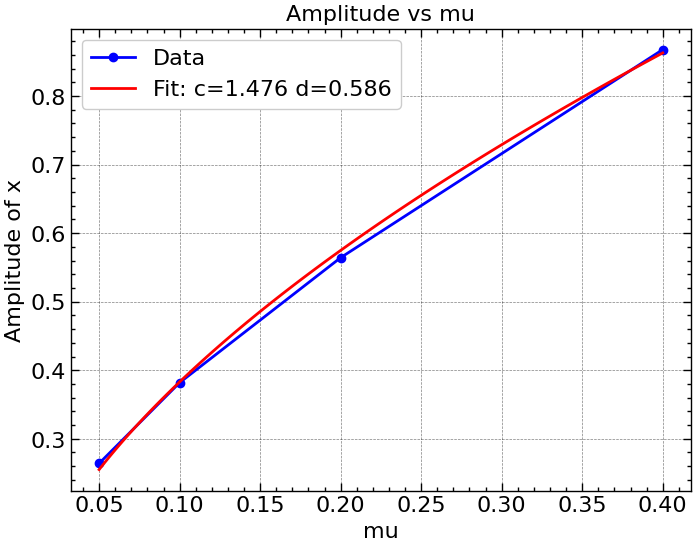
\includegraphics[width=0.75\textwidth]{Figure_2.png}
	\caption{Amplitude as a function of the value of \(\mu\). The function \(y=c\cdot\mu^d\) is fitted. The resulting values aren't the exact theoretical value but are close enough. After all, we have 4 points to go off of.}
\end{figure}
\subsubsection{Period}
The period calculated for \(\mu=0.05\) is \(6.3\). The expectation was \(T=2\pi/a=2\pi=6.28\) so it's again pretty good.